\begin{figure}[!htbp]
\centering
    \begin{minipage}{0.9\columnwidth}
        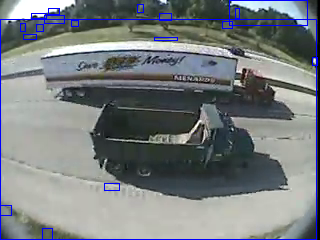
\includegraphics[width=0.48\linewidth, height = 0.3\linewidth]{./img/bg/252707.png}
        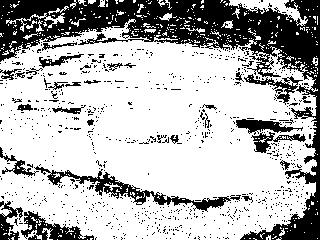
\includegraphics[width=0.48\linewidth, height = 0.3\linewidth]{./img/bg/252707_FG.png}
        \subcaption{Camera auto-exposure.}
        \label{subfig:bg-autoExposure}
    \end{minipage}
    \hspace{0.02\columnwidth}
    \begin{minipage}{0.9\columnwidth}
        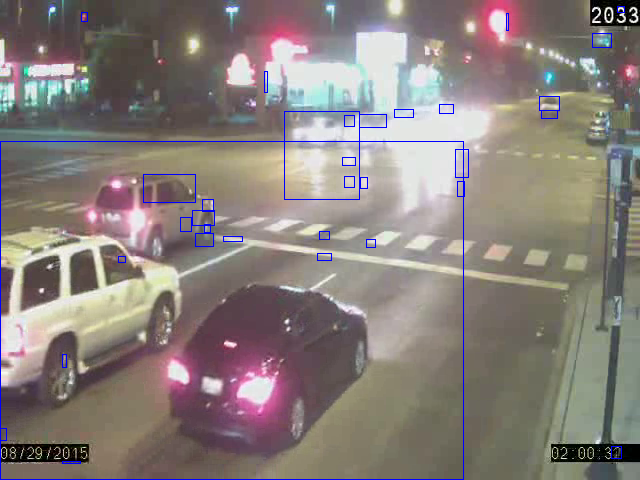
\includegraphics[width=0.48\linewidth, height = 0.3\linewidth]{./img/bg/ciceroPeterson.png}
        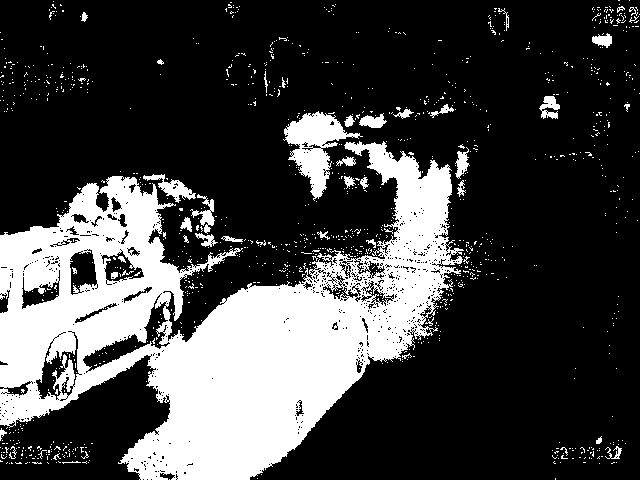
\includegraphics[width=0.48\linewidth, height = 0.3\linewidth]{./img/bg/ciceroPeterson_FG.png}
        \subcaption{Illumination change.}
        \label{subfig:bg-illuminationChange}
    \end{minipage}
    \vfill
    \begin{minipage}{0.9\columnwidth}
        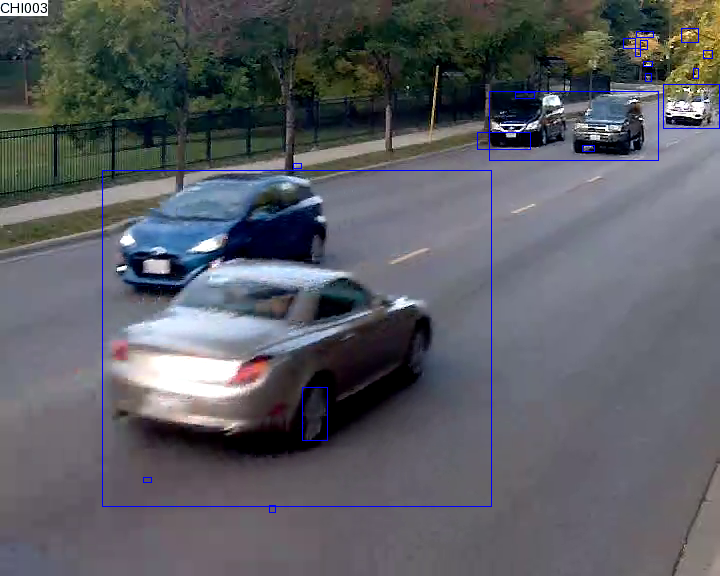
\includegraphics[width=0.48\linewidth, height = 0.3\linewidth]{./img/bg/ILCHI_CHI003.png}
        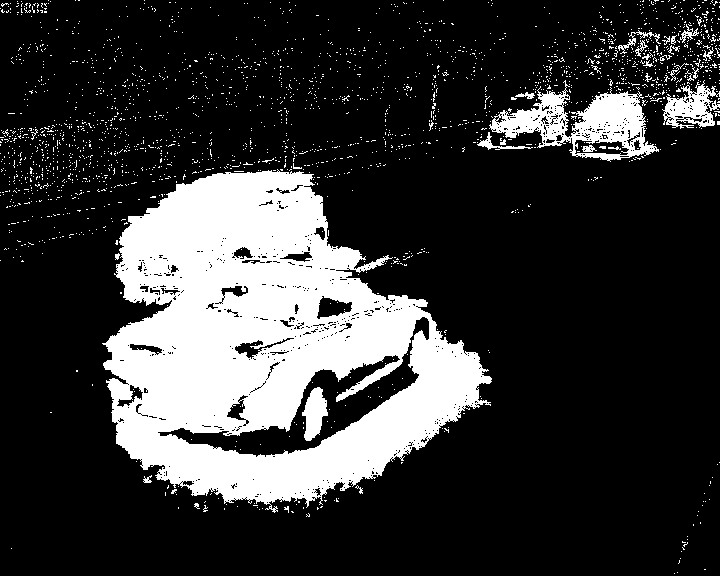
\includegraphics[width=0.48\linewidth, height = 0.3\linewidth]{./img/bg/ILCHI_CHI003_FG.png}  
        \subcaption{Occlusion. Note also the shadow, due to illumination change.} 
        \label{subfig:bg-occlusion}
    \end{minipage}
    \hspace{0.02\columnwidth}
    \begin{minipage}{0.9\columnwidth}
        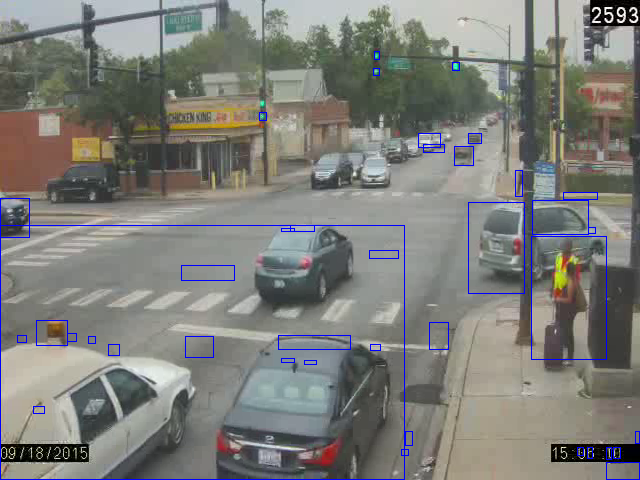
\includegraphics[width=0.48\linewidth, height = 0.3\linewidth]{./img/bg/halsted.png}
        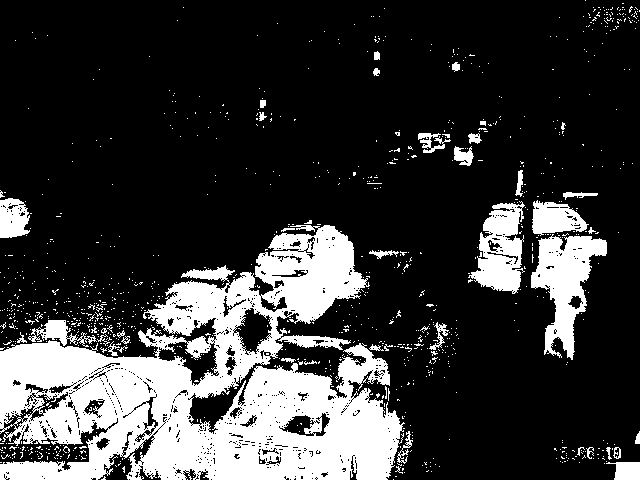
\includegraphics[width=0.48\linewidth, height = 0.3\linewidth]{./img/bg/halsted_FG.png}  
        \subcaption{Ghosting. Vehicles stopped at red light have become part of the background model.} 
        \label{subfig:bg-ghost}
    \end{minipage}
    %\vspace{-0.5em}
    \caption{Common background subtraction failure cases. Pixel values change for many reasons other than motion.}
    \label{fig:tracker-bg}
\end{figure}